%% For submission and review of your manuscript please change the
%% command to \documentclass[manuscript, screen, review]{acmart}.
%%
%% When submitting camera ready or to TAPS, please change the command
%% to \documentclass[sigconf]{acmart} or whichever template is required
%% for your publication.
%%
%%
\documentclass[sigplan,review,dvipsnames,screen,10pt]{acmart}

\usepackage{listings}
\usepackage{agda}
% \usepackage{bbm}
\usepackage{mathpartir}
\usepackage{tikz}
\usetikzlibrary{positioning}

\newcommand{\LamWhatif}{\ensuremath{\lambda^{1/2}_{\hookleftarrow}}}
\newcommand{\LamOurs}{\ensuremath{\lambda^{1/2!}_{\hookleftarrow}}}

% \usepackage{dsfont}
% \usepackage{bbm}
\usepackage{bbold}
\usepackage{newunicodechar}

\DeclareFontEncoding{LS1}{}{}
\DeclareFontSubstitution{LS1}{stix}{m}{n}
\DeclareSymbolFont{symbols2}{LS1}{stixfrak}{m}{n}
\DeclareMathSymbol{\typecolon}{\mathbin}{symbols2}{"25}

\newunicodechar{λ}{\ensuremath{\mathnormal\lambda}}
\newunicodechar{σ}{\ensuremath{\mathnormal\sigma}}
\newunicodechar{τ}{\ensuremath{\mathnormal\tau}}
\newunicodechar{π}{\ensuremath{\mathnormal\pi}}
\newunicodechar{ℕ}{\ensuremath{\mathbb{N}}}
\newunicodechar{∷}{\ensuremath{::}}
\newunicodechar{≡}{\ensuremath{\equiv}}
\newunicodechar{≅}{\ensuremath{\cong}}
\newunicodechar{∀}{\ensuremath{\forall}}
\newunicodechar{ᴸ}{\ensuremath{^L}}
\newunicodechar{ᴿ}{\ensuremath{^R}}
\newunicodechar{ʳ}{\ensuremath{^r}}
\newunicodechar{ⱽ}{\ensuremath{^V}}
\newunicodechar{⟧}{\ensuremath{\rrbracket}}
\newunicodechar{⟦}{\ensuremath{\llbracket}}
\newunicodechar{⊤}{\ensuremath{\top}}
\newunicodechar{⊥}{\ensuremath{\bot}}
\newunicodechar{₁}{\ensuremath{_1}}
\newunicodechar{₂}{\ensuremath{_2}}
\newunicodechar{₃}{\ensuremath{_3}}
\newunicodechar{₄}{\ensuremath{_4}}
\newunicodechar{₅}{\ensuremath{_5}}
\newunicodechar{₆}{\ensuremath{_6}}
\newunicodechar{₇}{\ensuremath{_7}}
\newunicodechar{₈}{\ensuremath{_8}}
\newunicodechar{₉}{\ensuremath{_9}}
\newunicodechar{∈}{\ensuremath{\in}}
\newunicodechar{₀}{\ensuremath{_0}}
\newunicodechar{′}{\ensuremath{'}}
\newunicodechar{ˢ}{\ensuremath{^S}}
\newunicodechar{ᴬ}{\ensuremath{^A}}
\newunicodechar{∘}{\ensuremath{\circ}}
% \newunicodechar{𝟙}{\ensuremath{\mathds{1}}}  
% \newunicodechar{𝟘}{\ensuremath{\mathds{O}}}
% \newunicodechar{𝟙}{\ensuremath{\mathbbm{I}}}  
\newunicodechar{𝟘}{\ensuremath{\mathbb{O}}}
\newunicodechar{ᴾ}{\ensuremath{^P}}
\newunicodechar{ᵀ}{\ensuremath{^T}}
\newunicodechar{⊎}{\ensuremath{\uplus}}
\newunicodechar{ι}{\ensuremath{\iota}}
\newunicodechar{⇐}{\ensuremath{\Leftarrow}}
\newunicodechar{⇒}{\ensuremath{\Rightarrow}}
\newunicodechar{∎}{\ensuremath{\mathnormal\blacksquare}}
\newunicodechar{➙}{\ensuremath{\to^P}}
\newunicodechar{Δ}{\ensuremath{\Delta}}
\newunicodechar{∅}{\ensuremath{\emptyset}}
\newunicodechar{⁺}{\ensuremath{^+}}
\newunicodechar{𝕏}{\ensuremath{\mathbb{X}}}
%\newunicodechar{·}{\ensuremath{\cdot}} %seems to be defined already!
\newunicodechar{∙}{\ensuremath{\bullet}}
\newunicodechar{⁇}{\ensuremath{?}}
\newunicodechar{‼}{\ensuremath{!}}
\newunicodechar{⊕}{\ensuremath{\oplus}}
\newunicodechar{ℤ}{\ensuremath{\mathbb{Z}}}
\newunicodechar{μ}{\ensuremath{\mu}}
\newunicodechar{∃}{\ensuremath{\exists}}
\newunicodechar{⨟}{\ensuremath{\fatsemi}}
\newunicodechar{Σ}{\ensuremath{\Sigma}}
\newunicodechar{ᵣ}{\ensuremath{_r}}
\newunicodechar{ᵢ}{\ensuremath{_i}}
\newunicodechar{≢}{\ensuremath{\nequiv}}
\newunicodechar{≟}{\ensuremath{\stackrel{{\tiny?}}{=}}}
\newunicodechar{≤}{\ensuremath{\le}}
\newunicodechar{ᵇ}{\ensuremath{^b}}
\newunicodechar{𝓣}{\ensuremath{\mathcal{T}}}
\newunicodechar{𝓔}{\ensuremath{\mathcal{E}}}
\newunicodechar{Γ}{\ensuremath{\Gamma}}
\newunicodechar{γ}{\ensuremath{\gamma}}
\newunicodechar{⊔}{\ensuremath{\sqcup}}
\newunicodechar{α}{\ensuremath{\alpha}}
\newunicodechar{η}{\ensuremath{\eta}}
\newunicodechar{ω}{\ensuremath{\omega}}
\newunicodechar{◁}{\ensuremath{\lhd}}
%PT: seems to be already defined
%\newcommand{\lambdabar}{{\mkern0.75mu\mathchar '26\mkern -9.75mu\lambda}}
\newunicodechar{ƛ}{\ensuremath{\lambdabar}}
\newunicodechar{Λ}{\ensuremath{\mathnormal\Lambda}}
\newunicodechar{ρ}{\ensuremath{\rho}}
\newunicodechar{𝓖}{\ensuremath{\mathcal{G}}}
\newunicodechar{ℓ}{\ensuremath{\ell}}
\newunicodechar{♯}{\ensuremath{\sharp}}
\newunicodechar{⇓}{\ensuremath{\Downarrow}}
\newunicodechar{𝓥}{\ensuremath{\mathcal{V}}}
\newunicodechar{∧}{\ensuremath{\wedge}}
\newunicodechar{ₛ}{\ensuremath{_s}}
\newunicodechar{χ}{\ensuremath{\chi}}
\newunicodechar{⊨}{\ensuremath{\models}}
\newunicodechar{⦂}{\ensuremath{\typecolon}}
\newunicodechar{ς}{\ensuremath{\varsigma}}
\newunicodechar{𝓓}{\ensuremath{\mathcal{D}}}
\newunicodechar{∎}{\ensuremath{\square}}
\newunicodechar{■}{\ensuremath{\blacksquare}}
\newunicodechar{↠}{\ensuremath{\twoheadrightarrow}}
\newunicodechar{↪}{\ensuremath{\hookrightarrow}}
\newunicodechar{β}{\ensuremath{\beta}}
\newunicodechar{ξ}{\ensuremath{\xi}}
\newunicodechar{𝟙}{\ensuremath{\mathbb{1}}}
\newunicodechar{𝟚}{\ensuremath{\mathbb{2}}}
\newunicodechar{≔}{\ensuremath{:=}}
\newunicodechar{𝓢}{\ensuremath{\mathcal{S}}}
\newunicodechar{⊢}{\ensuremath{\vdash}}
\newunicodechar{∋}{\ensuremath{\ni}}
\newunicodechar{ₕ}{\ensuremath{_h}}
\newunicodechar{ᵥ}{\ensuremath{_v}}
\newunicodechar{≼}{\ensuremath{\preceq}}
\newunicodechar{𝓗}{\ensuremath{\mathcal{H}}}
\newunicodechar{⊣}{\ensuremath{\dashv}}
\newunicodechar{ᶜ}{\ensuremath{^c}}
\newunicodechar{″}{\ensuremath{''}}
\newunicodechar{‴}{\ensuremath{'''}}
\newunicodechar{ₙ}{\ensuremath{_n}}
\newunicodechar{∣}{\ensuremath{\mid}}
\newunicodechar{⁗}{\ensuremath{''''}}
\newunicodechar{ʰ}{\ensuremath{^h}}
\input{agda-generated}
\newcommand\Aamp{\AgdaFunction{\ensuremath{\&}}}
\newcommand\Att{\AgdaInductiveConstructor{tt}}
\newcommand\Ado{\AgdaKeyword{do}}
\newcommand\AZ{\AgdaDatatype{ℤ}}
\newcommand\Asuc{\AgdaInductiveConstructor{suc}}
\newcommand\Azero{\AgdaInductiveConstructor{zero}}
\newcommand\Anat{\AgdaInductiveConstructor{nat}}
\newcommand\Aint{\AgdaInductiveConstructor{int}}
\newcommand\Abool{\AgdaInductiveConstructor{bool}}
\newcommand\Atend{\AgdaInductiveConstructor{end}}
\newcommand\Atsend[2]{\AgdaInductiveConstructor{‼{\textcolor{black}{\ensuremath{#1}}}∙{\textcolor{black}{\ensuremath{#2}}}}}
\newcommand\Atrecv[2]{\AgdaInductiveConstructor{⁇{\textcolor{black}{\ensuremath{#1}}}∙{\textcolor{black}{\ensuremath{#2}}}}}
\newcommand\Atcfsend[1]{\AgdaInductiveConstructor{‼{\textcolor{black}{\ensuremath{#1}}}}}
\newcommand\Atcfrecv[1]{\AgdaInductiveConstructor{⁇{\textcolor{black}{\ensuremath{#1}}}}}
\newcommand\Atcfcomp[2]{\AgdaInductiveConstructor{{\textcolor{black}{\ensuremath{#1}}}⨟{\textcolor{black}{\ensuremath{#2}}}}}
\newcommand\Atcfskip{\AgdaInductiveConstructor{skip}}
\newcommand\ACSKIP{\AgdaInductiveConstructor{SKIP}}
\newcommand\ACEND{\AgdaInductiveConstructor{END}}
\newcommand\ACCLOSE{\AgdaInductiveConstructor{CLOSE}}
\newcommand\ACfork{\AgdaInductiveConstructor{fork}}
\newcommand\ACconnect{\AgdaInductiveConstructor{connect}}
\newcommand\ACterminate{\AgdaInductiveConstructor{terminate}}
\newcommand\ACdelegateIN{\AgdaInductiveConstructor{delegateIN}}
\newcommand\ACdelegateOUT{\AgdaInductiveConstructor{delegateOUT}}
\newcommand\ACtransmit{\AgdaInductiveConstructor{transmit}}
\newcommand\ACbranch{\AgdaInductiveConstructor{branch}}
\newcommand\ACclose{\AgdaInductiveConstructor{close}}
\newcommand\ACSEND{\AgdaInductiveConstructor{SEND}}
\newcommand\ACRECV{\AgdaInductiveConstructor{RECV}}
\newcommand\ACSELECT{\AgdaInductiveConstructor{SELECT}}
\newcommand\ACCHOICE{\AgdaInductiveConstructor{CHOICE}}
\newcommand\AXCommand{\AgdaDatatype{XCmd}}
\newcommand\ACommand{\AgdaDatatype{Cmd}}
\newcommand\ACommandStack{\AgdaDatatype{CmdStack}}
\newcommand\ASession{\AgdaDatatype{Session}}
\newcommand\ASplit{\AgdaDatatype{Split}}
\newcommand\AMSession{\AgdaDatatype{MSession}}
\newcommand\ASet{\AgdaDatatype{Set}}
\newcommand\ASetOne{\AgdaDatatype{Set$_1$}}
\newcommand\ASeto{\AgdaDatatype{Setω}}
\newcommand\Abinaryp{\AgdaFunction{binaryp}}
\newcommand\Aunaryp{\AgdaFunction{unaryp}}
\newcommand\ACheck{\AgdaFunction{Check}}
\newcommand\ACausality{\AgdaFunction{Causality}}
\newcommand\ACheckDual{\AgdaFunction{CheckDual0}}
\newcommand\Aexecutor{\AgdaFunction{exec}}
\newcommand\Aexec{\AgdaFunction{exec}}
\newcommand\AIO{\AgdaFunction{IO}}
\newcommand\Amu{\AgdaInductiveConstructor{\ensuremath{\mu}}}
\newcommand\AMU{\AgdaInductiveConstructor{LOOP}}
\newcommand\AUNROLL{\AgdaInductiveConstructor{UNROLL}}
\newcommand\ACONTINUE{\AgdaInductiveConstructor{CONTINUE}}
\newcommand\Aback{\AgdaInductiveConstructor{\ensuremath{`}}}
\newcommand\Amanyunaryp{\AgdaFunction{many-unaryp}}
\newcommand\Arestart{\AgdaFunction{restart}}
\newcommand\ASerialize{\AgdaRecord{Serialize}}
\newcommand\ARawMonad{\AgdaRecord{RawMonad}}
\newcommand\AReaderT{\AgdaRecord{ReaderT}}
\newcommand\AStateT{\AgdaRecord{StateT}}
\newcommand\Aput{\AgdaFunction{put}}
\newcommand\Amodify{\AgdaFunction{modify}}
\newcommand\Aget{\AgdaFunction{get}}
\newcommand\Aproject{\AgdaFunction{project}}
\newcommand\AlocateSplit{\AgdaFunction{locate-split}}
\newcommand\Aadjust{\AgdaFunction{adjust}}
\newcommand\Aid{\AgdaFunction{id}}
\newcommand\AprimSend{\AgdaFunction{primSend}}
\newcommand\AprimRecv{\AgdaFunction{primRecv}}
\newcommand\Aleafp{\AgdaFunction{leafp}}
\newcommand\Abranchp{\AgdaFunction{branchp}}
\newcommand\Atreep{\AgdaFunction{treep}}
\newcommand\AIntTreeF{\AgdaFunction{IntTreeF}}
\newcommand\ACLeaf{\AgdaInductiveConstructor{Leaf}}
\newcommand\ACBranch{\AgdaInductiveConstructor{Branch}}
\newcommand\AtoN{\AgdaFunction{toℕ}}
\newcommand\Asplit{\AgdaFunction{split}}
\newcommand\AisValue{\AgdaDatatype{isValue}}
\newcommand\AValue{\AgdaDatatype{Value}}
\newcommand\Ajoin{\AgdaFunction{join}}
\newcommand\AExpr{\AgdaDatatype{Expr}}
\newcommand\AVar{\AgdaDatatype{Var}}
\newcommand\ACExpr{\AgdaFunction{CExpr}}
\newcommand\Acont{\AgdaFunction{cont}}
\newcommand\Adollar{\AgdaOperator{\AgdaFunction{\AgdaUnderscore{}\$\AgdaUnderscore{}}}}
\newcommand\AVSem{\AgdaOperator{\AgdaFunction{𝓥⟦\AgdaUnderscore{}⟧}}}
\newcommand\AESem{\AgdaOperator{\AgdaFunction{𝓔⟦\AgdaUnderscore{}⟧}}}
\newcommand\AESemx[1]{\AgdaOperator{\AgdaFunction{𝓔⟦#1⟧}}}
\newcommand\ADSemx[1]{\AgdaOperator{\AgdaFunction{𝓓⟦#1⟧}}}
\newcommand\AGSem{\AgdaOperator{\AgdaDatatype{𝓖⟦\AgdaUnderscore{}⟧}}}
\newcommand\ATSem{\AgdaOperator{\AgdaDatatype{𝓣⟦\AgdaUnderscore{}⟧}}}
\newcommand\Ainn{\AgdaDatatype{inn}}
\newcommand\ADEnv{\AgdaDatatype{Env\ensuremath{^*}}}
\newcommand\AapplyEnv{\AgdaFunction{apply-env}}
\newcommand\Alookup{\AgdaFunction{lookup}}
\newcommand\AREL{\AgdaFunction{REL}}
\newcommand\ARelEnv{\AgdaFunction{RelEnv}}
\newcommand{\AV}{\AgdaFunction{𝓥}}
\newcommand{\Asubst}{\AgdaFunction{subst}}
\newcommand{\Asubstlo}{\AgdaFunction{substl$\omega$}}
\newcommand{\Acong}{\AgdaFunction{cong}}
\newcommand{\Atrans}{\AgdaFunction{trans}}
\newcommand{\Arefl}{\AgdaInductiveConstructor{refl}}
\newcommand{\AValueDown}{\AgdaFunction{Value-\ensuremath{\Downarrow}}}
\newcommand{\AGLookup}{\AgdaFunction{𝓖-lookup}}
\newcommand{\ACsubClosed}{\AgdaFunction{Csub-closed}}
\newcommand{\ATsubClosed}{\AgdaFunction{Tsub-closed}}
\newcommand{\Ahere}{\AgdaInductiveConstructor{here}}
\newcommand{\Athere}{\AgdaInductiveConstructor{there}}
\newcommand{\Atskip}{\AgdaInductiveConstructor{tskip}}
\newcommand{\ATwk}{\AgdaFunction{Twk}}
\newcommand{\Anull}{\AgdaInductiveConstructor{∅}}
\newcommand{\ATRen}{\AgdaFunction{TRen}}
\newcommand{\ATSub}{\AgdaFunction{TSub}}
\newcommand{\ATren}{\AgdaFunction{Tren}}
\newcommand{\ATsub}{\AgdaFunction{Tsub}}
\newcommand{\ATliftR}{\AgdaFunction{Tliftᵣ}}
\newcommand{\ATliftS}{\AgdaFunction{Tliftₛ}}
\newcommand{\ATidR}{\AgdaFunction{Tidᵣ}}
\newcommand{\ATidS}{\AgdaFunction{Tidₛ}}
\newcommand{\AERen}{\AgdaFunction{ERen}}
\newcommand{\AESub}{\AgdaFunction{ESub}}
\newcommand{\AEren}{\AgdaFunction{Eren}}
\newcommand{\AEsub}{\AgdaFunction{Esub}}
\newcommand{\AEliftR}{\AgdaFunction{Eliftᵣ}}
\newcommand{\AEliftS}{\AgdaFunction{Eliftₛ}}
\newcommand{\AEliftRL}{\AgdaFunction{Eliftᵣ-l}}
\newcommand{\AEliftSL}{\AgdaFunction{Eliftₛ-l}}
\newcommand{\AEidR}{\AgdaFunction{Eidᵣ}}
\newcommand{\AEidS}{\AgdaFunction{Eidₛ}}
\newcommand{\AFusionTSubTSub}{\AgdaFunction{fusion-TSub-TSub}}
\newcommand{\AFusionESubESub}{\AgdaFunction{fusion-ESub-ESub}}
\newcommand{\ALRVsub}{\AgdaFunction{LRVsub}}
\newcommand{\AEEsingleSubstPreserves}{\AgdaFunction{EEsingle-subst-preserves}}
\newcommand{\AETsingleSubstPreserves}{\AgdaFunction{ETsingle-subst-preserves}}


\newcommand\AOne{\AgdaInductiveConstructor{𝟙}}
\newcommand\ATwo{\AgdaInductiveConstructor{𝟚}}
\newcommand\AType{\AgdaDatatype{Type}}
\newcommand\AqBounded{\AgdaDatatype{q-Bounded}}
\newcommand\AQType{\AgdaDatatype{QType}}
\newcommand\ACTAbs{\AgdaInductiveConstructor{TAbs}}
\newcommand\ACRef{\AgdaInductiveConstructor{Ref}}
\newcommand\ACref{\AgdaInductiveConstructor{ref}}
\newcommand\AClam{\AgdaInductiveConstructor{lam}}
\newcommand\ACFun{\AgdaInductiveConstructor{Fun}}
\newcommand\ACTVClos{\AgdaInductiveConstructor{TVClos}}
\newcommand\ACTVRef{\AgdaInductiveConstructor{TVRef}}
\newcommand\AInt{\AgdaDatatype{Int}}
\newcommand\AEnv{\AgdaDatatype{Env}}
\newcommand\AWellformed{\AgdaDatatype{Wellformed}}



\newcommand*\ACode[1]{\AgdaFontStyle{#1}}
\newcommand*\AField[1]{\AgdaField{#1}}
\newcommand*\ACon[1]{\AgdaInductiveConstructor{#1}}
\newcommand*\AKw[1]{\AgdaKeyword{#1}}
\newcommand*\AFun[1]{\AgdaFunction{#1}}
\newcommand*\ACom[1]{\AgdaComment{#1}}


%%% Local Variables:
%%% mode: latex
%%% TeX-master: "second-class"
%%% End:



%% Rights management information.  This information is sent to you
%% when you complete the rights form.  These commands have SAMPLE
%% values in them; it is your responsibility as an author to replace
%% the commands and values with those provided to you when you
%% complete the rights form.

% \copyrightyear{2025}
% \acmYear{2025}
% \setcopyright{cc}
% \setcctype{by}
% \acmConference[OLIVIERFEST '25]{Proceedings of the Workshop Dedicated to Olivier Danvy on the Occasion of His 64th Birthday }{October 12--18, 2025}{Singapore, Singapore}
% \acmBooktitle{Proceedings of the Workshop Dedicated to Olivier Danvy on the Occasion of His 64th Birthday (OLIVIERFEST '25), October 12--18, 2025, Singapore, Singapore}\acmDOI{10.1145/3759427.3760373}
% \acmISBN{979-8-4007-2150-2/2025/10}

%%% The following is specific to OLIVIERFEST '25 and the paper
%%% 'What I Always Wanted to Know about Second Class Values'
%%% by Peter Thiemann.
%%%
\setcopyright{cc}
\setcctype{by}
\acmDOI{10.1145/3759427.3760373}
\acmYear{2025}
\copyrightyear{2025}
\acmISBN{979-8-4007-2150-2/25/10}
\acmConference[OLIVIERFEST '25]{Proceedings of the Workshop Dedicated to Olivier Danvy on the Occasion of His 64th Birthday}{October 12--18, 2025}{Singapore, Singapore}
\acmBooktitle{Proceedings of the Workshop Dedicated to Olivier Danvy on the Occasion of His 64th Birthday (OLIVIERFEST '25), October 12--18, 2025, Singapore, Singapore}
\received{2025-07-15}
\received[accepted]{2025-07-31}



%%
%% Submission ID.
%% Use this when submitting an article to a sponsored event. You'll
%% receive a unique submission ID from the organizers
%% of the event, and this ID should be used as the parameter to this command.
%%\acmSubmissionID{123-A56-BU3}


\begin{document}

\title{What I Always Wanted to Know About Second Class Values}

%%
%% The "author" command and its associated commands are used to define
%% the authors and their affiliations.
%% Of note is the shared affiliation of the first two authors, and the
%% "authornote" and "authornotemark" commands
%% used to denote shared contribution to the research.
\author{Peter Thiemann}
\email{thiemann@acm.org}
\orcid{0000-0002-9000-1239}
\affiliation{%
  \institution{University of Freiburg}
  \city{Freiburg}
  \country{Germany}
}

\begin{abstract}
Second class values are allocated on the run-time stack and they may contain pointers
to other values on the stack. They were first discussed in connection with the
infamous funarg problem, but then forgotten as heap-allocated closures were
discovered.

Recent work has resurrected the interest in second class values as they allow us
to safely allocate some data structures (e.g., closures) on the run-time stack.
This approach has the advantage of avoiding the cost and the
unpredictable timing of garbage collection for
these structures as their deallocation takes no extra time when the
stack is popped. 
A system with qualified types ensures that second class values do not
escape across stack pops.

We take a second look at this work and extend/modify their formal framework
with first-class and second-class references in the style of ML. Along
the way we answer a question that left us mystified in the previous
work:  What, exactly, is the meaning of a type qualifier? 
\end{abstract}

%%
%% The code below is generated by the tool at http://dl.acm.org/ccs.cfm.
%% Please copy and paste the code instead of the example below.
%%
\begin{CCSXML}
<ccs2012>
<concept>
<concept_id>10011007.10011006.10011008.10011009.10011012</concept_id>
<concept_desc>Software and its engineering~Functional languages</concept_desc>
<concept_significance>300</concept_significance>
</concept>
<concept>
<concept_id>10003752.10010124.10010125.10010130</concept_id>
<concept_desc>Theory of computation~Type structures</concept_desc>
<concept_significance>500</concept_significance>
</concept>
<concept>
<concept_id>10011007.10011006.10011039.10011311</concept_id>
<concept_desc>Software and its engineering~Semantics</concept_desc>
<concept_significance>500</concept_significance>
</concept>
</ccs2012>
\end{CCSXML}

\ccsdesc[300]{Software and its engineering~Functional languages}
\ccsdesc[500]{Theory of computation~Type structures}
\ccsdesc[500]{Software and its engineering~Semantics}
\keywords{Second class values, functional programming, stack
  allocation, qualified types}

%%
%% This command processes the author and affiliation and title
%% information and builds the first part of the formatted document.
\maketitle
\lstset{language=python,morekeywords={Array,SArray},literate=
  {->1}{{\ensuremath{\rightarrow^1}}}3
  {->2}{{\ensuremath{\rightarrow^2}}}3}

\section{Introduction}

When the implementation of functional programming languages was still
an art, implementors were struggling to make all values ``first
class''. In particular, function values. In this context, first
class means that a function can be passed as an argument to another
function, returned as a result, or stored in a data structure. Thus,
it is a key feature to enable full-fledged higher-order programming.

Soon, implementors ran into the funarg problem \cite{moses70:_funct_lisp_funar}. This problem arises
when a function is passed as an argument or returned from a function
call. The issue is that the function in transit may refer to free
variables, and when the function leaves its defining scope, these free
variables become dangling references. 

Here is an example in Lisp.
\begin{lstlisting}[language=lisp]
(defun make-adder (x)
  (lambda (y) (+ x y)))

(setq add5 (make-adder 5))
(add5 3) ; => 8
\end{lstlisting}
The call to \lstinline|(make-adder 5)| creates a stack frame that
contains the binding \texttt{x = 5}. If the \lstinline|lambda| were just
returned as an expression, it would contain a dangling reference to
\texttt{x} because the stack is popped after the call.\footnote{When
  we say ``the stack is popped'' we usually mean that the topmost
  stack frame is discarded.}

This example is an instance of the \emph{upward funarg problem}
(return a function). The
dual \emph{downward funarg problem} (pass a function as a parameter)
is usually not a problem 
because the values that function bodies refer to are still available
on the stack. Pascal \cite{jensen91:_pascal} is a language that implemented this design:
functions can be passed downwards, but not returned. 

The well-known solution to the problem is representing functions by
closures that contain an environment with copies of the values of all
free variables besides the function body (or the code pointer in
compiled code) \cite{landin66,DBLP:conf/acm/Reynolds72}.
Usually, a closure is a heap-allocated data structure because its
lifetime can exceed the defining scope---indeed, for addressing the
upward funarg problem, it is a requirement that the closure can escape
from its defining scope.

Unfortunately, excessive heap allocation puts stress on the garbage
collector whereas memory management for stack-allocated data comes
(almost) for free. This idea was pushed to its limits by the seminal work on
region-based memory management
\cite{DBLP:conf/popl/TofteT94,DBLP:journals/iandc/TofteT97}. In
practice, the situation is not so clear cut as allocation with
Cheney's two-space collector or with generational collectors is also
very cheap \cite{DBLP:journals/jfp/AppelS96}. However, segments of code that are provably free of
garbage collection have deterministic timing and can satisfy hard
timing constraints, as they are certainly not interrupted by garbage
collection. 

Recent work on second class values
\cite{DBLP:conf/oopsla/OsvaldEWAR16} has
added a new, low cost angle to this subject. In this work, the authors
propose a qualified type system that categorizes values as first-class
or second-class with the rough intutition that first-class values are
heap allocated. This work has subsequently been refined in the core
calculus $\LamWhatif$
\cite{DBLP:conf/ecoop/XhebrajB0R22}, where functions are
either represented by heap closures or by stack closures. Invoking a
heap closure pushes a new frame on the stack and discards it on return from the
closure. Invoking a stack closure merely extends the current stack
frame and this extension is \emph{not} discarded on return.
This model enables writing code that can locally allocate data on the
stack as long as it does not escape from the most recently invoked
heap closure.

\begin{figure}[tp]
  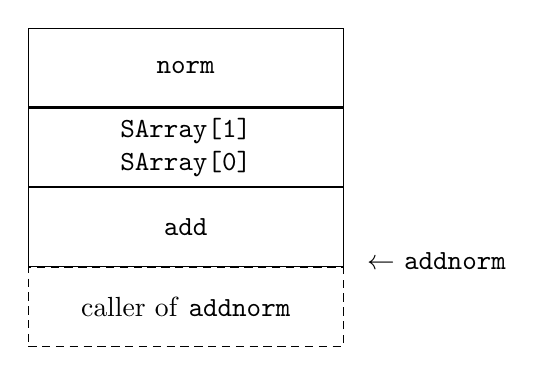
\begin{tikzpicture}[
  box/.style={draw, minimum width=4cm, minimum height=1cm, align=center, inner sep=0pt},
  ghost/.style={draw, densely dashed, minimum width=4cm, minimum height=1cm},
  arr/.style={->, thick}
]

% Stack boxes directly on top of each other
\node[box] (norm) {\texttt{norm}};
\node[box, below=0pt of norm] (sarray) {\texttt{SArray[1]} \\ \texttt{SArray[0]}};
\node[box, below=0pt of sarray] (add) {\texttt{add}};
\node[ghost, below=0pt of add] (dots) {caller of \texttt{addnorm}}; % Dashed ghost box for continuation
\node[right= 20pt of add] (refnode) {};
\node[below= 2pt of refnode] (addnorm) {\quad\quad $\leftarrow$ \texttt{addnorm}};

\end{tikzpicture}
\caption{Run-time configuration}
  \label{fig:runtime-configuration}
\end{figure}
This idea extends to stack allocation of data structures
other than closures. Here is an example using arrays (in Python-style syntax):
\begin{lstlisting}
def add(l: Array[int],
        r: Array[int]
       ) ->2 SArray[int]:
    return SArray[l[0]+r[0], l[1]+r[1]]
def norm (arr: SArray[int]) ->2 int:
    return arr[0]*arr[0] + arr[1]*arr[1]
def addnorm (l: Array[int],
             r: Array[int]) ->1 int:
    return norm (add(l, r))
\end{lstlisting}
Let's assume that type \texttt{Array} is
allocated on the heap while \texttt{SArray} is stack-allocated.
Assume further that \texttt{addnorm} is a heap closure while \texttt{add}
and \texttt{norm} are stack closures as indicated by the annotations
on the arrows.
In this configuration, \texttt{add} can safely allocate the
\texttt{SArray} on the run-time stack.

Here is what happens when invoking \texttt{addnorm} on two lists, step by step.
\begin{enumerate}
\item Create a new stack frame with arguments \lstinline|l| and
  \lstinline|r|.
\item Extend the stack frame to call \texttt{add}.
\item The function \texttt{add} allocates the
  \texttt{SArray} in the current stack frame and returns
  \emph{without discarding the frame}.
\item Extend the stack frame to call \texttt{norm}; the argument
  points to the \texttt{SArray} in the stack frame.
\item Return the result of \texttt{norm} \emph{without discarding the
    frame}.
\item Finally, return the result and pop the stack thus discarding the frame(s) for
  \texttt{addnorm}, \texttt{add}, and \texttt{norm}.
\end{enumerate}
The illustration in Figure~\ref{fig:runtime-configuration} shows the
stack configuration right before the last step. The dashed ghost frame
at the bottom belong to the caller of \texttt{addnorm}. The stack
frame for \texttt{addnorm} contains the frames for \texttt{add} and
\texttt{norm}, as well as the stack-allocated array.

In the rest of the paper, we introduce a call-by-value lambda calculus $\LamOurs$
with second class functions and second class references, which can
express a computation just like the one for \texttt{addnorm}. Our
calculus~$\LamOurs$ is heavily inspired by~$\LamWhatif$, but it
implements some subtle changes and one major extension.

\begin{itemize}
\item Like $\LamWhatif$, $\LamOurs$ comes with a qualified type system
  that classifies values into first and second class.
\item Our calculus $\LamOurs$ implements a slightly more realistic encoding of stack frames
  than $\LamWhatif$ because it pushes arguments of stack closures on
  the stack and accesses them by pointers into the stack. In contrast, the formal model of
  $\LamWhatif$ apparently copies relevant parts of the stack.
\item The calculus $\LamOurs$ extends $\LamWhatif$ by mutable references that can
  be safely allocated on the stack or on the heap. This extension
  requires a subtle change in the type system compared to $\LamWhatif$
  (see Section~\ref{sec:types} for discussion). 
\end{itemize}
The definition of $\LamOurs$ and its type soundness proof are fully
mechanized in Agda
\cite{DBLP:conf/afp/Norell08,team25:_agda_homep}. The source code is
separately available in a GitHub
repository\footnote{\url{https://github.com/peterthiemann/what-if.git}}. 
The main body of this paper contains and comments on excerpts of this
mechanized development. We expect readers to be reasonably fluent with
Agda's syntax. 

% In the conclusions, we return to the questions raised in the abstract.
% \begin{itemize}
% \item What, exactly, is the meaning of a type qualifier?  
% \item Can we implement this scheme with a type-based, selective CPS
%   translation?
% \item Can we extend the formal framework of previous work
%   with first-class and second-class references?
% \end{itemize}

\section{Syntax}
\label{sec:syntax}

\subsection{Qualifiers}
\label{sec:qualifiers}

Qualifiers $q$ are used throughout in types and
expressions. The intuition is that qualifier {\AOne} classifies heap-related ``things'' and {\ATwo} classifies
stack-related ``things''.  They show up in the syntax of
types and expressions and also as indices for the evaluation
judgment. Qualifiers come with two, subtly different, semantics which
we make more precise in each case and discuss in the conclusion.
\Qual

Type qualifiers form a complete lattice with lattice order~$\le$. We
prove that $\le$ is a partial order and that evidence for the order is unique.

\subsection{Types}
\label{sec:types}



Qualified types are defined by mutual recursion between $\AType$ and
$\AQType$ ranged over by $T$ and $S$, respectively:
\begin{align*}
  T &::= \ACUnit \mid \ACBase \mid \ACFun~S~S \mid \ACRef~S & S & ::= T^q
\end{align*}
Type formation (judgment $\vdash S$) is non-trivial as it ensures the
type qualification is consistent, i.e.,
that types are meaningful. We write $S\le q'$ as a shorthand for
$S=T^q$ and $q\le q'$.
\begin{mathpar}
  \inferrule{}{\vdash \ACUnit^q} \and
  \inferrule{}{\vdash \ACBase^q} \and
  \inferrule{\vdash S_1 \\ \vdash S_2 \\ S_1 \le q \\ S_2
    \le q}{\vdash (\ACFun~S_1~S_2)^q} \and
  \inferrule{\vdash S \\ S \le q}{\vdash (\ACRef~S)^q}
\end{mathpar}
The following Agda definitions express the same constraints, but
yield intrinsically consistent type qualifications because they formalize the type
formation judgment $\vdash S$. 
\QType
The $\AQType$ only manages the qualifier and defines the type indexed
by the qualifier. The $\AType$ comprises the unit type, base type,
function and reference type.

\subsection{Design Rationale}
\label{sec:design-rationale}


To understand the consistency constraints on qualifiers, we have to understand the
underlying data model. We call a value of type $T^{\AOne}$ a
\emph{heap value}. We can generally think of such a value as a 
heap address, which points to a heap record that contains the actual
data. Similarly, a \emph{stack value} is represented by a stack
address and the value \emph{contains} whatever is stored at that
address. (There are exceptions: values of type {\ACUnit} and {\ACBase} 
are unboxed, i.e., directly represented.)

Specifically, the constraint for $\ACRef$ enforces that a heap
value cannot contain a stack value. Otherwise, a heap record would
contain a stack address which would be able to escape its defining scope.
The constraint for $\ACFun$ ensures that a heap-allocated function
only has heap values as arguments and as results. This (quite
conservative) restriction means that stack addresses are invalidated
once a heap-allocated function pushes a new stack frame.

The earlier calculus $\LamWhatif$ does not impose either of these
constraints: references are not supported by $\LamWhatif$ and we are
forced to restrict function types like this because we added
references.

Let's consider an example to see the need for this
restriction. Generally, if we pass a stack value to a heap closure,
then we need to ensure that the callers' stack does not get
corrupted. In $\LamWhatif$, there is no problem, but references may
corrupt the stack.

Concretely, consider a stack value $r : \ACRef~\ATwo~(\ACRef~\ATwo~\AInt)$ which contains
another stack value which points  to a number and suppose we can pass that value
to a heap-allocated closure. The call to this heap closure creates a new
stack frame, which gets discarded on return from the closure.
Suppose now, the body of the closure creates a new stack value on the
local stack as in $x =
\ACref~\ATwo~(42)$ of type $x : \ACRef~\ATwo~\AInt$.
The typing allows us to update $r$ with this fresh reference as in $r
:= x$. But now the callers' stack contains an address into the current stack
frame, which becomes invalid after returning from the heap closure (which
discard the top-most stack frame).

We chose a simple approach to avoid this situation by disallowing 
stack values as arguments to heap
closures, which is enforced by the consistency constraints for
function types. The recent literature contains several reports that consider
less constrained (but vastly more complex) systems (e.g.,
\cite{DBLP:journals/pacmpl/BaoWBJHR21,DBLP:journals/pacmpl/LorenzenWDEL24}),
and we leave further exploration of design 
alternatives to future work.

\subsection{Expressions}
\label{sec:expressions}

Variables are slightly special as they are indexed with a qualifier,
which is intended to provide an upper bound of the class of the value
bound to the variable. Identifiers \AFun{Ident} are just strings.
\Variables

The syntax of expressions is standard. Two constructors take
qualifiers as arguments. The qualifier in the $\ACref$ constructor directs allocation
to the heap or to the stack. The qualifiers in the $\AClam$
constructor to mark the class of the argument and the return value,
but do no govern allocation of the closure itself.
\Expr


\section{Run-Time Objects}
\label{sec:run-time-objects}

\begin{figure}[tp]
  \Values
  \caption{Run-time objects}
  \label{fig:run-time-objects}
\end{figure}

The operational semantics manipulates four kinds of run-time objects
with mutually recursive definitions: values $\AVal$, environments
$\AEnv$, stacks $\AStack$, and
heaps $\AHeap$ (Fig.~\ref{fig:run-time-objects}). 

An environment of type $\AEnv$ is either empty, or it is extended with
a \emph{heap binding} $x:=v$ containing the value, or a \emph{stack binding} $x \Rightarrow a$, in which case the
environment contains the address $a$ of the value
in the (current) stack frame.

A value is either unit, constant, closure, or reference. Unit and
constants are directly representend. A closure is (morally) a pointer
to data stored according to the closure's qualifier $q$ ($\AOne$ heap,
$\ATwo$ stack). Our model elides this pointer because closures are
immutable (cf.\ \citet{DBLP:conf/ecoop/XhebrajB0R22}). We represent a
closure as a structure containing the
environment $\mathcal{E}$ with bindings for the free variables, the
stack $\mathcal{S}$ when the closure was created, the closure variable
$x$, the closure's body expression $e$, and the qualifier $q_r$ to
indicate the class of the return value. 

A reference value $\ACref~q~\ell$ is a true pointer.
Its qualifier $q$ indicates whether it is a heap or a stack
reference. The address $\ell$ either points to the heap or the current stack
frame, depending on $q$. 

Our model for the stack is bit unusual. From compiler construction,
one would expect a plain list of values which contains all currently
active stack frames with argument values and stack-allocated
references intertwined. However, for technical reasons (see
Section~\ref{sec:design-rationale}) we disallow stack pointers across
calls to heap-allocated closures. Therefore, we reset the stack
whenever we call a heap-allocated closure and accumulate new frames
(without popping) for calls to stack-allocated closures. On returning
from a heap-allocated closure, its call stack gets restored by the
operational semantic (Section~\ref{sec:evaluation}, rule
\ACEApp). Thus, our stack only contains the stack frame of the
currently active heap-allocated closure including nested calls to
stack-allocated closures.

To simplify the subsequent technical development, we also distinguish
between immutable and mutable parts of the stack. Hence, a stack
$\mathcal{S}$ consists of two lists of values. The list 
\texttt{vars} contains stack values referenced from the environment
(i.e., function arguments)
and the list \texttt{refs} contains ``memory cells'' to be used for
stack references.\footnote{Strictly speaking, we could collapse the
  two lists into one and represent a stack frame as a linear array of
  memory cells, but this structure is easier to deal with in the
  soundness proof.}

This rationale explains the stack extension relation and the operation
\AFun{new-frame?}. Extension is defined by pairing the prefix relation $\preceq$
on variables (their values do not change and their number does not
decrease) and $\le$ on the lengths of the references (their number
does not decrease).
\StackExtension

The \AFun{new-frame?} operation resets the stack to empty ($\mathcal{S}\emptyset$) when the
(closure) qualifier is $\AOne$ and keeps it, otherwise.
\NewFrame

A heap $\mathcal{H}$ is just a list of values, i.e., the
memory cells for heap references. 



\section{Typing}
\label{sec:typing}

As our operational semantics is a big-step semantics that relates
expressions to values, we need a typing relation for expressions and
also a value typing relation. Like
\citet{DBLP:conf/ecoop/XhebrajB0R22} we also include a subtyping
relation to make the system more flexible. Subtyping deals with the
situation where a function asks for an argument that can be put on the
stack, that is, the argument type has the form $T^{\ATwo}$. In this
situation, it is safe to pass a heap value of type $T^{\AOne}$ because
it is safe to put a heap pointer on the stack. Clearly, the converse
(putting a stack pointer on the heap) is unsafe and thus ruled out by
our system. Subtyping is a requirement in our system because all
elimination rules in the type system ask for second class values in
their elimination position (Section~\ref{sec:typing-rules}).

\subsection{Subtyping}
\label{sec:subtyping}
\begin{figure}[tp]
\begin{mathpar}
  \inferrule[\ACSUnit]{q_1 \le q_2}{\ACUnit^{q_1} <: \ACUnit^{q_2}} \and
  \inferrule[\ACSBase]{q_1 \le q_2}{\ACBase^{q_1} <: \ACBase^{q_2}} \and
  \inferrule[\ACSFun]{q_1 \le q_2 \\ S_3 <: S_1 \\ S_2 <: S_4 \\\\ S_1 \le q_1
    \\ S_2 \le q_1 \\ S_3 \le q_2 \\ S_4 \le q_2 }{(\ACFun~S_1~S_2)^{q_1} <:
    (\ACFun~S_3~S_4)^{q_2}} \and
  \inferrule[\ACSRef]{q_1 \le q_2 \\ S_1 <: S_2 \\ S_2 <: S_1 \\ S_1, S_2 \le q_1}{(\ACRef~S_1)^{q_1} <: (\ACRef~S_2)^{q_2}}
\end{mathpar}
  \caption{Subtyping}
  \label{fig:subtyping}
\end{figure}
\begin{figure}[tp]
  \SubtypingRelation  
  \caption{Subtyping (Agda)}
  \label{fig:subtyping-agda}
\end{figure}


Figure~\ref{fig:subtyping} contains the subtyping rules with the Agda
transcription in Figure~\ref{fig:subtyping-agda}. The traditional
rules contain the required consistency constraints which are implicit
in the Agda version. The {\ACSQual} rule is inlined in the traditional
rules with the constraint $q_1\le q_2$.

Subtyping
only concerns the qualifiers, while the overall structure of the types
remains the same. The rules are
structured in two mutually recursive layers, just like types. The
relation on $\AQType$ enables subsumption from heap values to stack
values: any heap pointer can be put on the stack, but not vice
versa. The relation on $\AType$ extends qualifier 
subtyping by enforcing contravariant and covariant
behavior for arguments and results of a function as well as invariant
behavior for values in a reference. Rule $\ACon{SQual}$ enforces that
the top-level qualifier can only be subsumed by a larger qualifier. This relation is taken from
\citet{DBLP:conf/ecoop/XhebrajB0R22}, but extended with reference types.

\subsection{Typing contexts}
\label{sec:typing-contexts}

Formation of typing contexts $\Gamma$ is as usual with a slight
twist. As variables are indexed by a qualifier, contexts contain an
equality that makes sure that the qualifier of a variable is the same
as the qualifier of the type it is bound to. The notation for an
extended context is $\Gamma, x:S[eq]$ where $eq$ enforces equal qualifiers.
\Contexts

Context lookup is standard. We use a straightforward variable
representation with explicit identifiers because we define the
semantics without recurse to substitution.
\ContextLookup

\subsection{Typing rules}
\label{sec:typing-rules}
\begin{figure}[tp]
  \TypingRules  
  \caption{Typing}
  \label{fig:typing}
\end{figure}
Figure~\ref{fig:typing} contains the typing rules. Most of them are
standard and unsurprising: type structure and qualifiers have to
match. Indeed, the rules $\ACTUnit$, $\ACTBase$, $\ACTAbs$, $\ACTApp$,
and $\ACTSub$ correspond to the rules in
\citet{DBLP:conf/ecoop/XhebrajB0R22}, with minor adaptations to deal
with consistency of qualified types.
Unit values and constants are never put on the stack, so their
qualifier does not matter. Rule {\ACTAbs} defines the typing of an
abstraction. The qualifier $q$ of the {\AClam} constructor determines
the class of the closure. The body of the lambda is typed in a
restricted typing context $\Gamma'$ which contains only the
bindings with class $\le q$ from the original context. This
restriction is enforced by the {\AqBounded} relation. The remaining
parts of the rule enforce the consistency of the type
qualification.

The rules $\ACTSeq$, $\ACTRef$, $\ACTDeref$, and $\ACTSetref$ deal
with sequencing and operations on references. They are new in this
work, but straightforward adaptations of the standard rules for
references to account for the qualifiers.

It is interesting to observe that all elimination positions in the
typing rules ask for second class values. This observation yields a
different interpretation of the qualifiers in types: A second class
value is never put on the heap. It is either directly consumed or
stored on the stack. In contrast, a first class value can be put on
the heap.

\subsection{Run-time typing}
\label{sec:run-time-typing}
\begin{figure}[tp]
  \ValueTyping
  \caption{Run-time typing}
  \label{fig:run-time-typing}
\end{figure}

Figure~\ref{fig:run-time-typing} contains the definitions for run-time
typing. The first relation formalizes value typing $\langle \Sigma_h,
\Sigma_s \rangle\vdash{[ v \typecolon S]}$ --- in heap type $\Sigma_h$
and stack type $\Sigma_s$, value $v$ has qualified type $S$. The
second relation formalizes agreement of context, run-time environment,
and stack: $\langle \Sigma_h , \Sigma_s,
\Gamma\rangle\models\mathcal{E}/\mathcal{S}$ --- in heap type
$\Sigma_h$, stack type $\Sigma_s$, and variable context $\Gamma$, we
have agreement with the run-time environment $\mathcal{E}$ and stack
$\mathcal{S}$.

Agreement consists of two components, $\models$-heap and
$\models$-stack.
Component $\models$-heap says that any variable binding of a heap variable to a
heap type in $\Gamma$ gives access to the value of this variable in
the run-time environment and the value has the type predicted by the
context.
Component $\models$-stack says that any binding of a stack variable to a type in
$\Gamma$ gives access to the stack address of this variable in the
run-time environment; moreover, looking up this address in the stack
succeeds and yields a value of the type predicted by the context.

Value typing for unit and constant is simple because they do not
depend on stack or heap.

Value typing for a closure in rule {\ACTVClos} contains a run-time
environment, but this run-time environment agrees with any stack that
is an extension of the creation stack $\mathcal{S}$ of the
closure. The qualifier $q$ determines the class of the closure; the
\AFun{new-frame?} operator returns the empty stack for a heap closure
and otherwise the identity. The  equality using \AFun{new-frame?}
ensures that the closure was created correctly (cf.\ Section~\ref{sec:run-time-objects}).
The context has to be $q$ bounded.
The body $e$ is typed with argument $S_1$ and result $S_2$.
The final subtyping judgment enables us retype the value with any
supertype.

Value typing for a reference in rule {\ACTVRef} dispatches on class
$q$ between the type environment $\Sigma_h$ for the heap and
$\Sigma_s$ for the stack. It affirms that the pointer $\ell$ is valid
(less than the length of the respective environment) and that looking
up the environment at $\ell$ yields the expected type $T$.
The final subtyping judgment also enable retyping with any supertype.

The rule is bit obfuscated because it is parameterized over some $T :
\AFun{Typeof}~q$, which is either a bare heap type (if $q=\AOne$) or a full qualified
type (if $q = \ATwo$). The \verb|^^| operators make up for the
difference as $\ACRef$ requires a full qualified type. Their
definition is technical but straightforward.

\subsection{Typing stacks and heaps }
\label{sec:typing-stacks-heaps}

Heap typing and stack typing are both straightforward. The typing
environment is a list of (heap) types which is pointwise related to a
list of values of the same length by the run-time value relation. Heap values do not
depend on stack values, so the stack type is not needed for typing a heap.

\HeapTyping
\StackTyping


\section{Evaluation}
\label{sec:evaluation}

We formalize evaluation in terms of an eight-place big-step evaluation
relation
$\mathcal{E}, \mathcal{H}, \mathcal{S} \vdash e \Downarrow{[ q ]} v
\dashv \mathcal{H}', \mathcal{S}'$ ---
in run-time environment $\mathcal{E}$ with heap $\mathcal{H}$ and
stack $\mathcal{S}$, the expression $e$ evaluates with target class
$q$ to value $v$, output heap $\mathcal{H}'$ and output stack
$\mathcal{S}'$.

There is exactly one evaluation rule for each
syntactic construct. This setup is different to $\LamWhatif$, where
all evaluation rules come in pairs, indexed by their class. Most of our
rules contain further case distinctions, which give rise to case
distinctions in the soundness proof. However, the same is true for
$\LamWhatif$ where both, the \textsc{EAppH} and \textsc{EAppS}, rules
cover two subcases directed by the value of $ptr$ (which may be $\bot$
or $k$) and the $\oplus$ operator, which dispatches on the class of
its argument. 

\RuleEUnit
Evaluation of a unit preserves heap and stack.

\RuleEVar
Variables are accessed through the environment. Heap variables yield
values, stack variables yield addresses, and the \AFun{decode}
function dereferences address on the stack, if needed.

\RuleEAbs
This rule distinguishes between heap allocated and stack allocated
closures guided by the annotation $q_1$. The former are created with
the empty stack $\mathcal{S}\emptyset$ while the latter
pick up the stack where they were created. The \AFun{q-bounded-Env}
relation removes binding with class greater than $q$ from the run-time
environment.

\RuleEApp
This rule deals with four cases at once. It distinguishes on $q$
between heap and stack closures and it distinguishes on $q_1$ between
heap and stack arguments. The former is handled by either creating a
new stack frame or reusing the existing one (function
\AFun{new-frame?} to start a frame and function \AFun{restore-frame?} to discard). The
latter is handled by the operators $\oplus$ which either adds a value
or its address to the run-time environment and $\oplus_s$ which
conditionally pushes a value on the stack.

Here we implement the rationale from
Section~\ref{sec:design-rationale}. The full stack is implicit in the
derivation of the evaluation judgment. At each call to a heap closure,
\AFun{new-frame?} creates a new, empty frame to execute the body of
the closure. After the call, it restores the previous frame.
A call to a stack closure always extends the current frame and leaves
it on the stack.


\RuleERef
To create a reference of class $q_1$, we evaluate its body at class
$q_1$. Then we either allocate it on the heap or on the stack and
leave the other component unchanged.

\RuleEDeref
We can evaluate the argument of deref at class $\ATwo$ because the
result is directly eliminated and never stored anywhere. Next, we either
read the value from the heap or from the stack depending on the class
of the reference.

\RuleESetref
We can evaluate the first argument of setref at class $\ATwo$ for the
same reason as before. The second is evaluated at class $q_1$ as
expected by the reference. The we either write to the heap or to the stack.

\RuleESeq
We evaluate the first subexpression of the sequence at class $\ATwo$
as its value is ignored.
Then we evaluate the second subexpression at the class $q$ expected by the context.

\section{Soundness}
\label{sec:soundness}
\begin{figure}[tp]
  \Wellformed
  \caption{Wellformedness}
  \label{fig:wellformedness}
\end{figure}
In preparation for the soundness proof, we need a notion of
\emph{wellformedness} which is a predicate on all run-time objects:
values, environments, stacks, and heaps. Wellformedness tells us that whenever
evaluation yields a stack closure, then the current stack is an
extension of the creation stack of the closure. Thus, it is safe to
continue using the closure because it cannot contain dangling references.

Figure~\ref{fig:wellformedness} contains the relevant definitions. In
the definition of the {\AWellformed} predicate on values, we apply
\AFun{clos-stack-env} to check if the value
is a closure and obtain its run-time environment $\mathcal{E}$ and its
creation-time stack $\mathcal{S}^c$. If the value is a heap value,
then the creation-time stack is empty and $\mathcal{E}$ is a pure heap
environment, which does not contain any stack bindings or stack
values. Furthermore, the current stack $\mathcal{S}$ is an 
extension of the creation-time stack and the run-time environment is
wellformed in both stacks.

A wellformed environment {\AWellformedEnv} contains only wellformed values and all heap
bindings are heap values.

Wellformedness extends pointwise to heaps and stacks (i.e., lists
of values; not shown).

\begin{figure}[tp]
  \SoundnessResult
  \caption{Results}
  \label{fig:soundness-result}
\end{figure}
The result of soundness is a record shown in
Figure~\ref{fig:soundness-result}.
It is parameterized over the input heap type, input stack type, the
return value $v$, its type $S$, the output heap $\mathcal{H}'$, and
the input and output stack $\mathcal{S}$ and $\mathcal{S}'$ of an
evaluation. It contains all relevant information to prove soundness by
induction on the evaluation relation.

Here are some highlights of the result.
\begin{itemize}
\item The output heap and output stack are well-typed extensions of
  the input heap and input stack of evaluation. The extensions of the
  typing assumptions for stack and heap are captured by
  ${\uparrow}\Sigma{\preceq_s}$ and  ${\uparrow}\Sigma{\preceq_h}$ and
  respective typing by ${\uparrow}{\vdash}\mathcal{S}$ and
  ${\uparrow}{\vdash}\mathcal{H}$.
\item The return value is (value) typed under the outgoing heap and
  stack types as stated in ${\uparrow}{\vdash} v$.
\item The output stack is an extension of the input stack (${\uparrow}\mathcal{S}{\preceq}$).
\item The return value is wellformed, as are the output heap and stack
  stated in ${\uparrow}\textsf{cls}$, ${\uparrow}\textsf{wf-}\mathcal{H}$ and ${\uparrow}\textsf{wf-}\mathcal{S}$.
\end{itemize}

\begin{figure}[tp]
  \EvalSoundness  
  \caption{Soundness theorem}
  \label{fig:soundness-theorem}
\end{figure}
Figure~\ref{fig:soundness-theorem} contains the statement of the
soundness theorem as proved. 
It states that all stack and heap accesses during evaluation of a
typed term are safe.
More precisely, suppose we are given a typed heap, a typed stack, and
an environment $\mathcal{E}$ that is admissible for some context
$\Gamma$ with this heap and stack type. Furthermore, all input
run-time objects (environment, heap, stack) are wellformed.
If we have an expression $e$ which has  type $S$ in context $\Gamma$,
and we evaluate $e$ under qualifier $q$ (which is an upper bound for
the qualification of $S$) to value $v$, then we obtain the result for the return
value $v$.

As the proof of the theorem is by induction on the evaluation relation
followed by inversion of the respective typing rule, we know that
every step of the evaluation is safe. In particular, value typing for
references enforces that there are no dangling stack references, which
is the point of the whole exercise.

\section{Conclusions}
\label{sec:conclusions}

As we demonstrate in this paper, it is possible to extend the prior
work \cite{DBLP:conf/ecoop/XhebrajB0R22} with first and second class
references. In Section~\ref{sec:types} we explain the differences
between $\LamWhatif$ and $\LamOurs$ in terms of wellformedness of
qualified types.

While we believe there is a less restrictive version of $\LamWhatif$
that eliminates wellformedness, it requires a careful and much more
complex design. We 
already discussed the issue with stack references of stack references,
but, of course, the same problem arises with (nested) stack closures
that contain stack references. Thus, a revised calculus would have a
significantly more complicated type system that keeps track of life
times and aliasing, probably along the lines of reachability types
\cite{DBLP:journals/pacmpl/BaoWBJHR21}. We leave this
exploration to future work.


To finish up, let's get back to the question raised in the abstract and
add another one that points to future work.

\subsection*{What, exactly, is the meaning of a type qualifier?}

The meaning depends on the respective purpose. The meaning for
\emph{specifying allocation} is $\AOne \to$ heap and $\ATwo \to$ stack. Another purpose
is to indicate a \emph{context of use} for a value. In this case $\AOne$
means ``this value may be put on the heap'' and $\ATwo$ means ``this
value will never be put on the heap'' (directly or indirectly).
\begin{itemize}
\item In types, the qualifier indicates the context of use.
\item In expressions, the type qualifier indicates the allocation site
  of references and closures. In a lambda expression $\AClam~q~ x~ e~
  q_1$, the second $q_1$ indicates the context of use for the body $e$
  of the lambda.
\item In values, the qualifier indicates the location where the value
  was allocated. In a closure, the second qualifier plays the same
  role as $q_1$ for lambda expressions.
\item In the evaluation judgment, the qualifier index $q$ denotes the
  context of use. This meaning can be derived from the way the
  constructs evaluate their elimination position in context $\ATwo$:
  these values will never be put on the heap, because they are
  destructed at this point of evaluation.
\end{itemize}

\subsection*{Can we implement this scheme with a type-based, selective CPS translation?}

Let's first clarify what we mean with this question. The classic
approach of compiling with continuations
\cite{DBLP:conf/acm/Steele77} goes (very roughly) like this:
Apply a wholesale translation to continuation-passing style (CPS) to the program, distinguish (local)
calls to continuations from serious function calls, implement the
former by jumps (reusing the stack frame) and the latter by full blown 
function calls that allocate fresh stack frames.

This approach can be implemented in an entirely heap-based manner
\cite{DBLP:books/cu/Appel1992}, but most compiler writers try to use
the stack to represent continuations for serious function calls. 

A little thought reveals that invocations of second class functions
live in between the jump and the full-blown function call. Hence, they
could be implemented by a jump combined with a stack-allocated
continuation. A 
possible tool for the first step in such an implementation of
$\LamOurs$ could be a selective CPS translation that \emph{does not}
transform calls to heap-allocated functions. This possibility
was hinted at in prior work \cite{DBLP:conf/ecoop/XhebrajB0R22},
\emph{but} for a version of $\LamWhatif$ \emph{without subtyping}.

In $\LamOurs$ with qualifier-driven subtyping, the type does not
convey enough information to determine the class of a closure. Indeed,
the typing rule for function application always expects a second-class
function of type $\ACFun~S_1~S_2~wf_1~wf_2~\hat{}~\ATwo$, but at run
time it could be a heap closure or a stack closure, as one can see
from the evaluation rule \ACon{EApp} for function application.

One strategy to address this situation would be to move from
set-theoretic subtyping to coercive subtyping
\cite{DBLP:conf/tacs/Reynolds91,DBLP:journals/logcom/Luo99}, where the
coercion at function types would correspond to eta expansion. The resulting
calculus would be amenable to a selective CPS translation, but one
would also have to discuss coherence of subsumption. We leave this
exploration to future work.

\subsection*{Can we extend the formal framework of previous work
  with first-class and second-class references?}

\begin{acks}
  Thanks to Julius Fischer for the many discussions on the subject. He
  implemented a prototype interpreter for $\LamOurs$ as part of his
  bachelor
  thesis.\footnote{\url{https://github.com/Proglang-Uni-Freiburg/LambdaCPS.git}}
  Thanks are also due to the reviewers who provided thoughtful
  feedback that improved the paper significanty.
  Thanks also to ChatGPT for drawing Figure~\ref{fig:runtime-configuration}.
\end{acks}

\section*{Data Availability Statement}
%%% To help readers understand the state of the intended artifact, we
%%% ask you to add a section just before references titled
%%% Data-Availability Statement in the initial submission. This will
%%% not count towards the page limit, but please limit it to at most a
%%% few paragraphs (usually one paragraph suffices). 

%%% In it, indicate whether an artifact exists, its nature and
%%% limitations, and whether it will be submitted for Artifact
%%% Evaluation. This section should ideally also include links to
%%% preliminary versions of (anonymized) artifacts, datasets, and so
%%% on that reviewers may find useful (but are not obliged to
%%% follow). The statement is not meant to be a detailed description
%%% of how to use the artifact; that should accompany the artifact
%%% itself. 

%%% It is understood that some papers have no artifacts but, given the
%%% broad range of what constitutes an artifact, it would be helpful
%%% to readers to explain why the paper has none. 

%%% Accepted papers that fail to provide an artifact after promising one will be asked to explain why they did not do so.

%%% Artifact Evaluation submission will closely follow paper
%%% notification, so make sure you check the Artifact Call as soon as
%%% you submit your paper. 

The Agda proof scripts are submitted as an artifact~\cite{thiemann25:_artif_what_i_alway_wanted}.


%%
%% The next two lines define the bibliography style to be used, and
%% the bibliography file.
\bibliographystyle{ACM-Reference-Format}
\bibliography{second-class}



\end{document}
\endinput
%%
%% End of file `second-class.tex'.
